\section{Theory}
% Delaunay-triangulering, punktsett, sirkelkriterie, distmesh (ikke 3D), etc.
In order to produce and use grid representations of the real world, there must be a way to map the real, continuous domain to a discrete representation. In order to get a general understanding of the following theory, we start by a couple generic definitions.

\begin{definition}[Point set]
A point set $P \in \mathbb{R}^n$ is a finite set of points in $\mathbb{R}^n$.
\end{definition}
While there exists infinite point sets, we limit ourself to finite sets.


\begin{definition}[Convex hull]
The convex hull of a point set $P$ is the minimal convex set containing $P$.
\end{definition}
\begin{figure}[h]
    \centering
    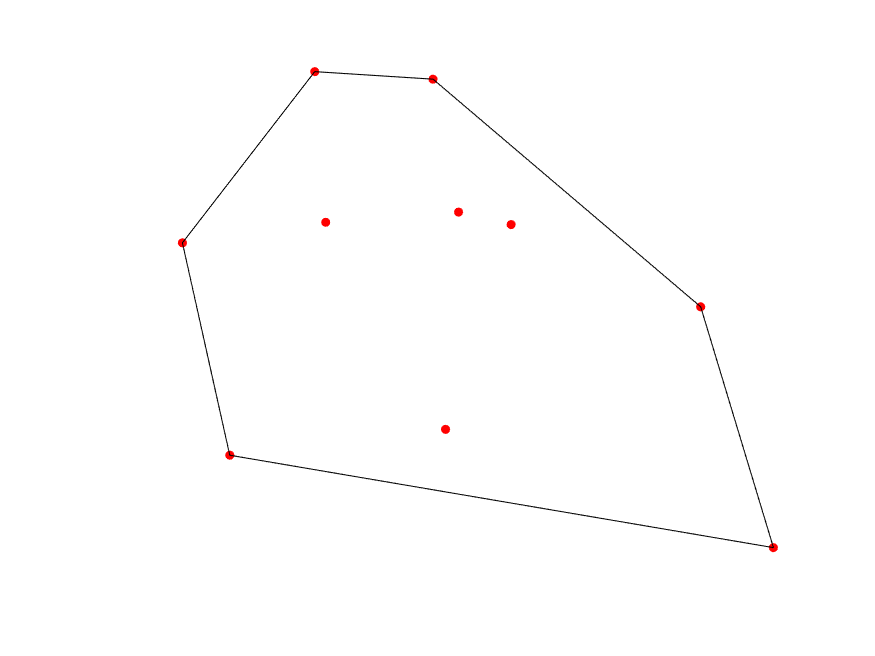
\includegraphics[width=0.5\textwidth]{report/Images/Theory/convex_hull.png}
    \caption[Example of a convex hull]{Example of a convex hull for a set of 10 randomly generated points in $\mathbb{R}^2$.}
    \label{fig:ex:convex_hull}
\end{figure}


\begin{definition}[Simplex]
A simplex is a generalization of a triangle to arbitrary dimensions.
\end{definition}
Simplices represent the simplest possible geometric object in a simple space. As grid representations of real scenarios are limited to three dimensions, we only need to consider the first four simplices:
\begin{itemize}
    \item A 0-simplex is a point,
    \item A 1-simplex is a line,
    \item A 2-simplex is a triangle,
    \item A 3-simplex is a tetrahedron.
\end{itemize}
In general, a $k$-simplex is a $k$-dimensional geometric object consisting of the convex hull of its $k + 1$ vertices.


\begin{definition}[Triangulation]
A triangulation $T$ of a point set $P$ is the set of simplices $T$ such that
\begin{itemize}
    \item The set of vertices in $T$ equals $P$
    \item The union of all simplices in $T$ equals the convex hull of $P$.
\end{itemize}
\end{definition}
\begin{figure}[h]
    \centering
    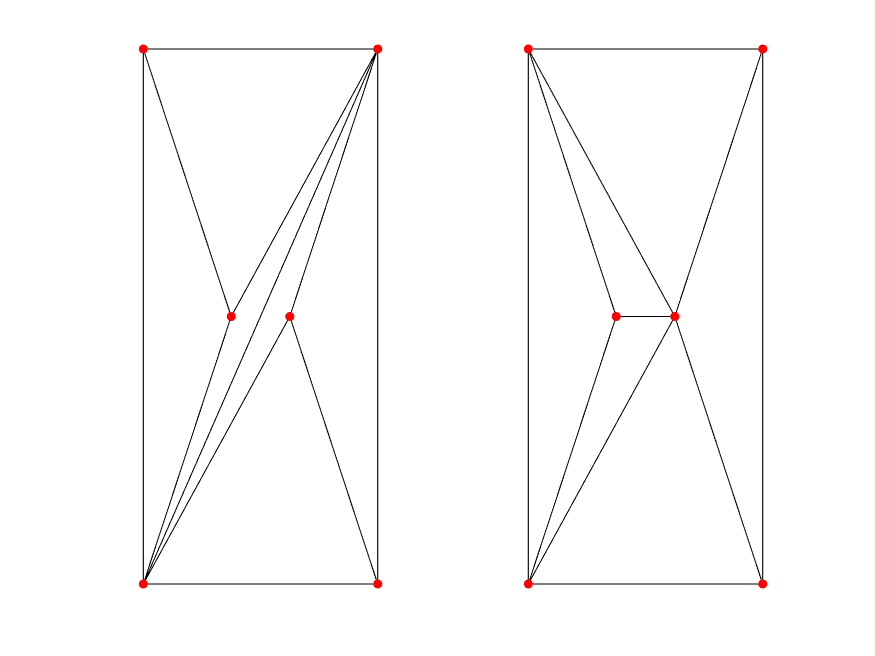
\includegraphics[width=0.7\textwidth]{report/Images/Theory/triangulation.png}
    \caption[Example of triangulation]{Example of two triangulations for a set of points $P \in \mathbb{R}^2$.}
    \label{fig:ex:triangulation}
\end{figure}

For a given point set, one can generally create multiple legal triangulations. \autoref{fig:ex:triangulation} shows two triangulations for the same point set $P$.


\subsection{Delaunay triangulation}
Delaunay triangulation is a triangulation first introduced by \textcite{delaunay_1943} in 1943. In order to understand Delaunay triangulation, we must first define the circumcircle.

\begin{definition}[Circumcircle]
A circumcircle of a polygon is a circle passing through all vertices of the polygon.
\end{definition}
\begin{figure}[ht]
    \centering
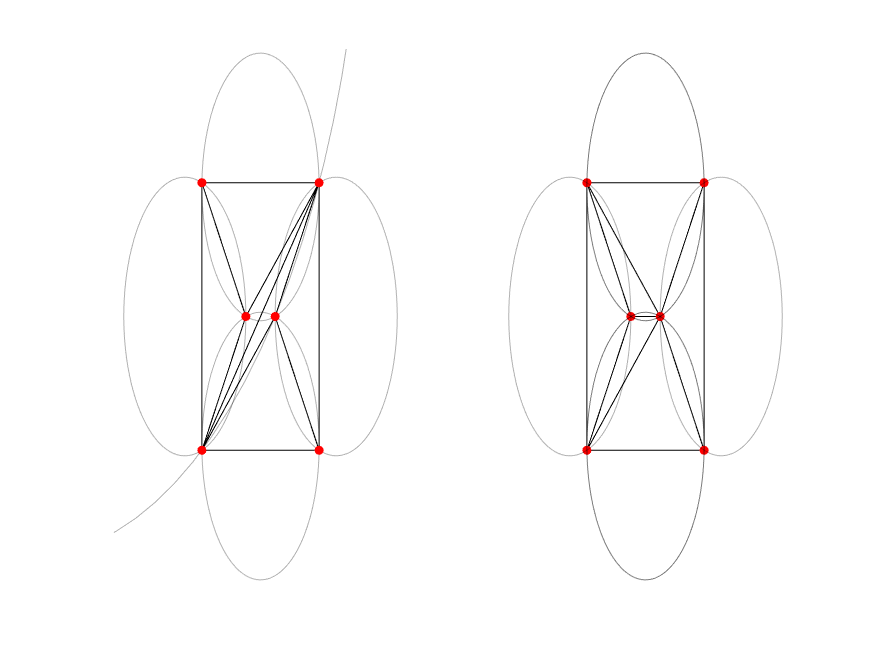
\includegraphics[width=0.8\textwidth]{report/Images/Theory/circumcircle.png}
    \caption[Example of circumcircles]{Example of circumcircles for the two triangulations in \autoref{fig:ex:triangulation}. Note that the leftmost plot has a been cropped.}
    \label{fig:ex:circumcircles}
\end{figure}

The Delaunay triangulation of a point set $P$ is defined as follows:
\begin{definition}
Let $T$ be a triangulation of the point set $P$. $T$ is a Delaunay triangulation if no vertices in $P$ are inside the circumcircle of any simplex in $T$.
\end{definition}

\subsection{Voronoi diagrams}


\subsection{Distmesh}

\subsection{PEBI grids}
\textcolor{red}{DETTE ER IKKE FERDIG}

\begin{equation}
    v_{s_i} = \left\{ x : x \in \mathbb{R}^d,\quad \abs{x - s_i} < \abs{x - s},\quad \forall s \in S \setminus \{s_i\} \right\}.
\end{equation}
The face between two sites, denoted by $v_{s_i, s_j}$ is made up by all points that are the same distant from two sites but further from any other sites, i.e.
\begin{equation}
    v_{s_i, s_j} = \left\{ x : x \in \mathbb{R}^d,\quad \abs{x - s_i} = \abs{x - s_j} < \abs{x - s},\quad \forall s \in S \setminus \{i, j\} \right\}.
\end{equation}

% Legg til en illustrasjon av PEBI